\section{Introduction}
\label{sec:introduction}

\begin{figure*}[t]
\centering
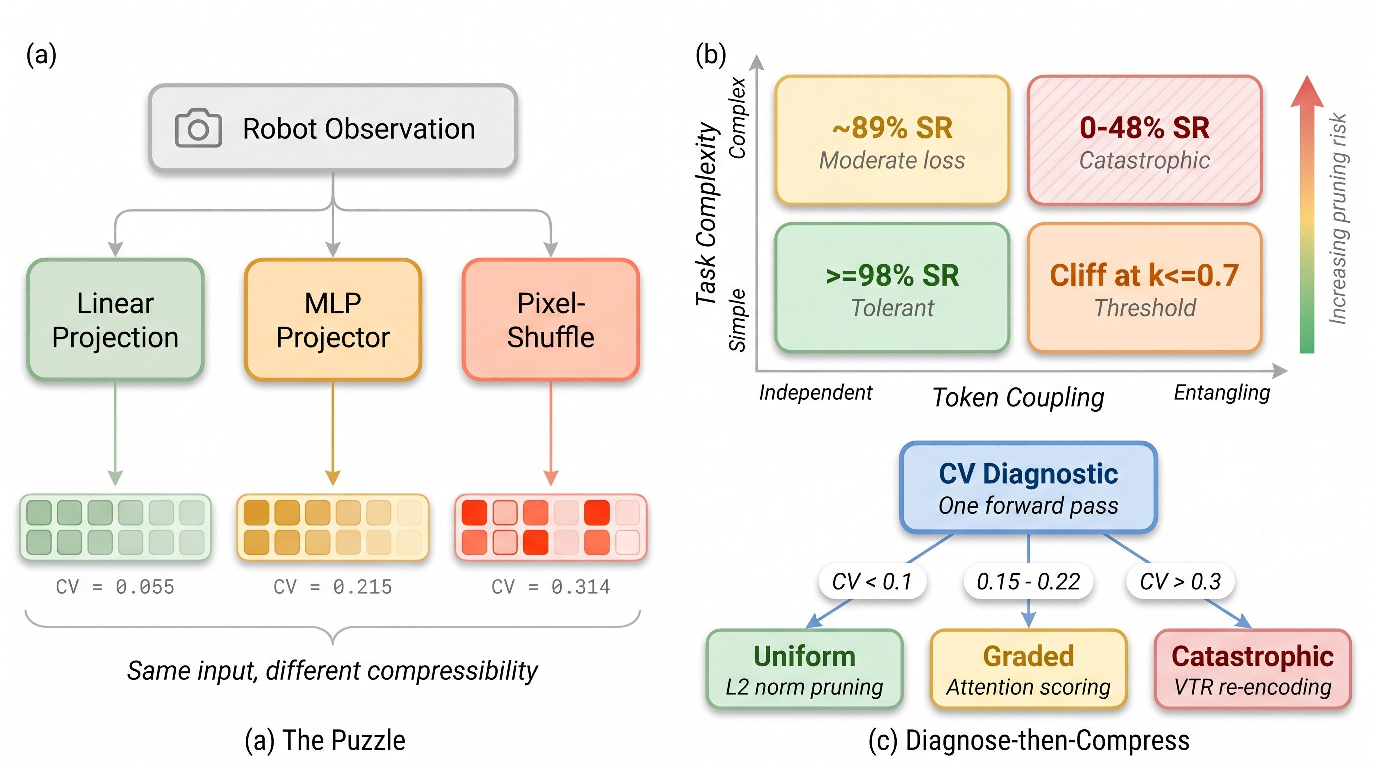
\includegraphics[width=\textwidth]{figures/paper/fig_hero_overview.pdf}
\caption{Overview of VLA token compressibility.
\textbf{(a)}~The same robot observation produces qualitatively different token importance patterns through different vision connectors, quantified by the coefficient of variation (CV) of post-connector token norms.
\textbf{(b)}~Connector architecture determines pruning tolerance: independent connectors degrade gracefully, entangling connectors exhibit cliffs; task complexity amplifies the divergence.
\textbf{(c)}~A single forward pass CV diagnostic routes each architecture to an appropriate compression strategy.}
\label{fig:teaser}
\end{figure*}

Vision-Language-Action (VLA) models process robot observations as hundreds of vision tokens, creating a computational bottleneck for real-time control. Token pruning, the removal of low-importance tokens before the language backbone, is well-established for vision transformers~\cite{rao2021dynamicvit,bolya2023tome,liang2022evit} and has been applied to VLAs~\cite{cheng2026vlaiap,xu2025vlacache,yang2025efficientvla,liu2025vlapruner}. Yet each method validates on a single architecture, implicitly assuming that pruning transfers across designs.

This assumption is unsafe. Current VLAs employ fundamentally different vision connectors (linear projections~\cite{black2024pi0}, MLP projectors~\cite{kim2024openvla}, pixel-shuffle folding~\cite{shukor2025smolvla}, and learned encoders with cross-token self-attention~\cite{zheng2025xvla}), each imposing distinct constraints on how visual information distributes across tokens. Whether a pruning strategy validated on one connector type will transfer to another is unknown; deploying it blindly risks silent degradation or complete failure.

We present the first cross-architecture study of VLA token compressibility, evaluating six architectures (450M--7B) across four LIBERO manipulation suites (Figure~\ref{fig:teaser}). The vision-language connector emerges as the strongest predictor of pruning robustness: token-independent connectors degrade gracefully, while token-entangling connectors exhibit catastrophic cliffs that task complexity amplifies. No scoring method is universally safe: importance-based selection can dramatically outperform or underperform random pruning depending on the connector, following an inverted-U importance margin that reverses at aggressive compression ratios. A zero-mask ablation isolates the mechanism: position disruption, not information loss, drives failure.

Our contributions: (1)~the first cross-architecture VLA compressibility analysis, revealing connector type as the dominant factor governing pruning tolerance; (2)~the coefficient of variation (CV) of post-connector token norms as a zero-cost, single-pass diagnostic predicting both pruning tolerance and scoring method sensitivity; (3)~mechanistic evidence that position disruption drives failure in position-sensitive architectures, plus a lightweight Vision Token Re-encoder (VTR, ${\sim}$5\% extra parameters) recovering baseline performance at 75\% compression for architectures where all deletion fails.
